\documentclass[titlepage]{article}
\newcommand\tab[1][1cm]{\hspace*{#1}}
\usepackage[left=12mm, top=12mm, right=12mm, bottom=12mm]{geometry}
\usepackage{gensymb}
\usepackage{float}
\usepackage{graphicx}
\usepackage{subcaption}

\begin{document}

\title{COMP 4107 Final Project\\
         {\small Clean vs. Raw Data performance on an LSTM chatbot system}}
\author{Lachlan Campbell, 100999056\\
              Elijah MacPherson, 100970225}
\maketitle

\section{Introduction}
\tab For this project we will attempt to implement a chatbox trained off of various transcript datasets. We will accomplish this using recurrent neural networks communicating and learning via sequence to sequence learning. The object of this project is to determine the effects of different data sets have on the conversational accuracy as well as training time. 

\section{Background}
In order to implement this chatbot we will be using LSTM (Long short-term memory) neural networks.
\begin{figure}[H]
	\centering
	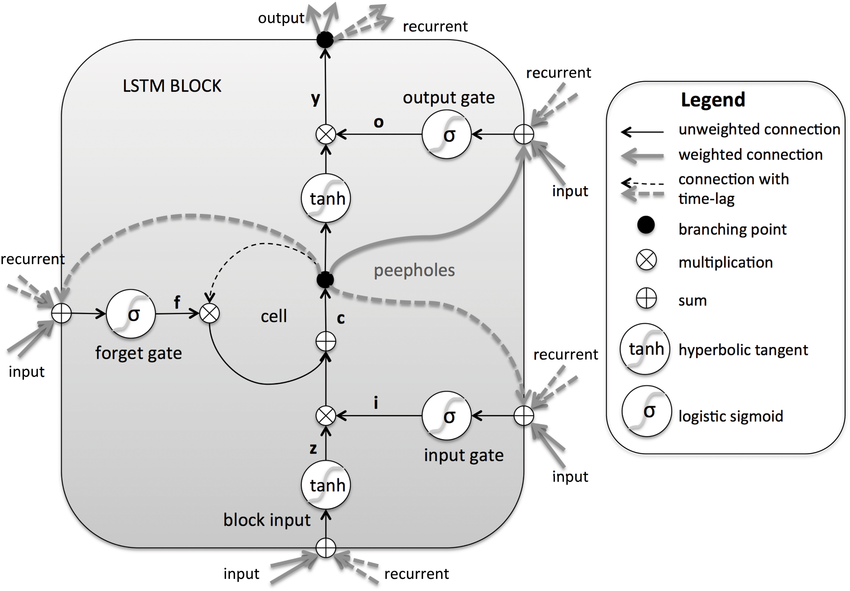
\includegraphics[width=120mm]{LSTM-model.png}
	\caption{An LSTM block recurrent neural network model.}
	\label{fig:lstm1}
\end{figure}
\begin{figure}[H]
	\centering
	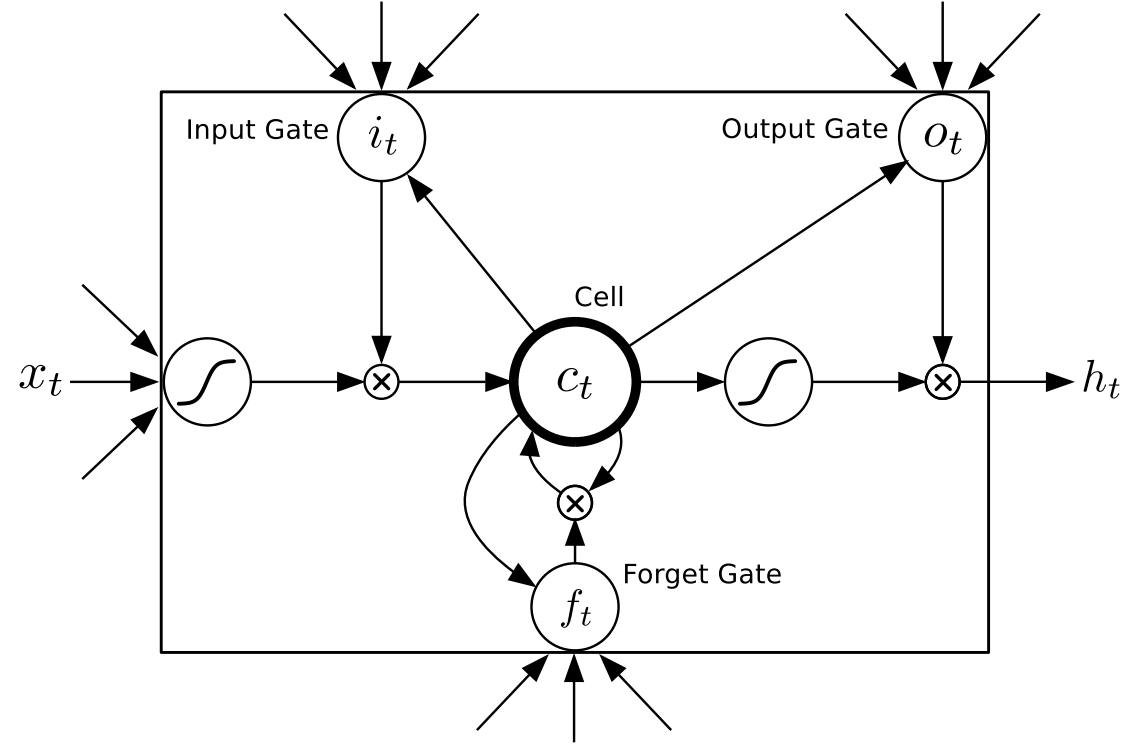
\includegraphics[width=120mm]{LSTM-model-2.png}
	\caption{A barebones view of the different gates involved in an LSTM.}
	\label{fig:lstm2}
\end{figure}
~\\~\\~\\~\\~\\	
\tab We will be using a method called sequence to sequence learning where two neural networks (namely an encoder NN and a decoder NN) communicate with each other in order to convert sequences from one domain to sequences in another domain. In our case we will be working within the domains of $statement\rightarrow reply$.
\begin{figure}[H]
	\centering
	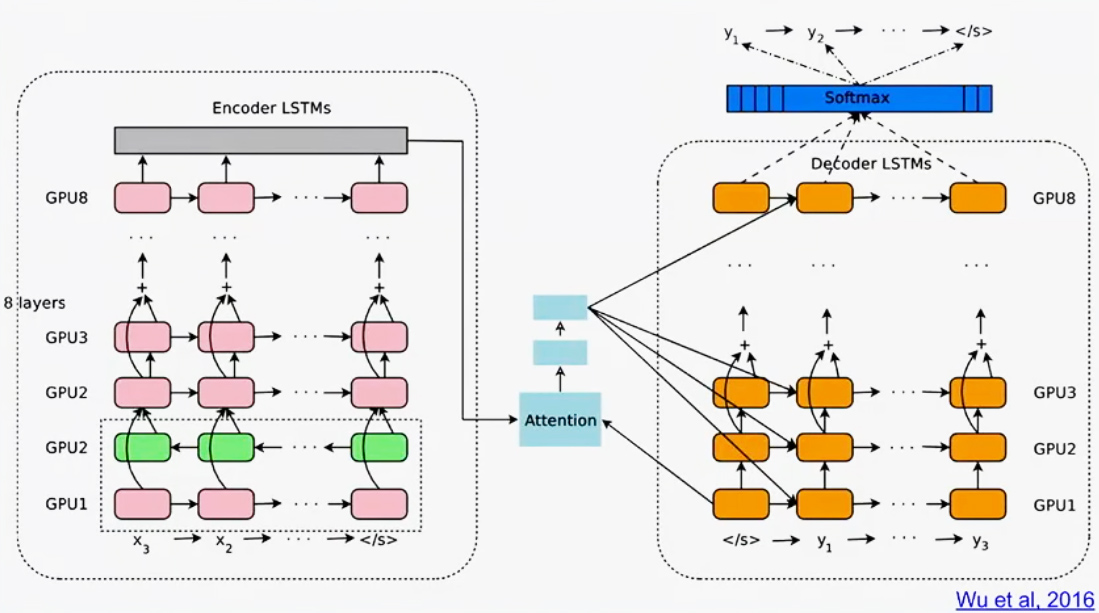
\includegraphics[width=120mm]{Seq2seq.jpg}
	\caption{A look at how google translate uses sequence to sequence learning to translate from one language to another}
	\label{fig:seq2seqgoogletranslate}
\end{figure}
The model above uses many LSTM's in the encoder NN and the decoder NN, but for the purposes of the project we will only be using one LSTM in each the encoder NN and the decoder NN.


\section{Problem Statement}
The aim of this project is to determine what the effects of a cleaned data set are on the:\\
\tab 1. Training time of an LSTM chatbot network\\
\tab 2. Overall proficiency at conversation.

\section{Results and Analysis}
Before training can begin, let us first look at the computational graph of our model:
\begin{figure}[H]
	\centering
	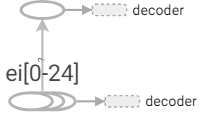
\includegraphics[width=120mm]{main_graph.png}
	\caption{The main graph of our chatbot network}
	\label{fig:maingraph}
\end{figure}
\begin{figure}[H]
	\centering
	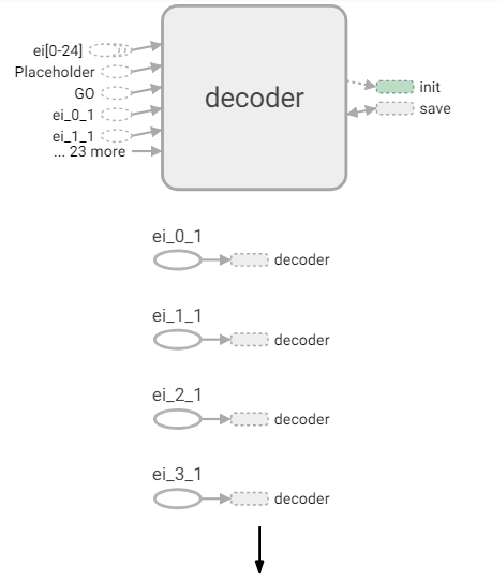
\includegraphics[width=120mm]{aux_nodes.png}
	\caption{A look at the auxilliary nodes of the model. Note there are 24 EI units in total.\\(extends below the arrow)}
	\label{fig:auxnodes}
\end{figure}

Training
\begin{figure}[H]
	\centering
	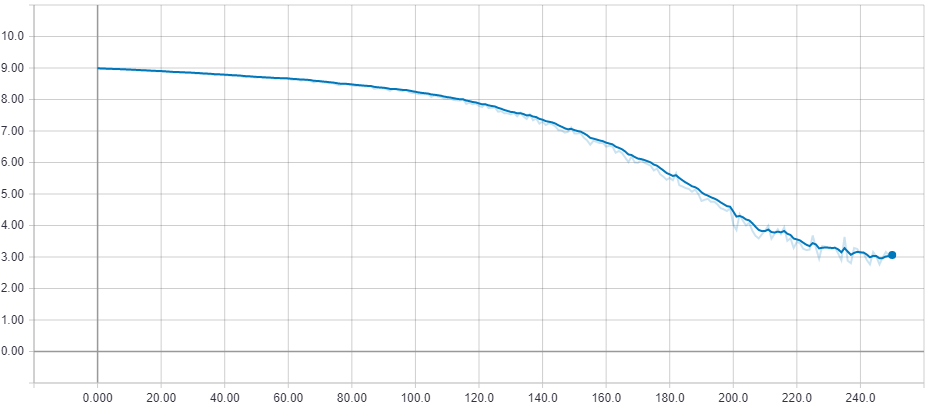
\includegraphics[width=120mm]{cost-clean-001.png}
	\caption{The cost function trained on a clean dataset with $\alpha = 0.001$}
	\label{fig:cc001}
\end{figure}
As you can see from the graph the cost seems to settle around 240 epochs with a minimum value of approx. 3.0.

\section{Conclusion}

\section{References}
\large{Works Cited:}\\
\small{

}
~\\~\\
\large{Images:}\\
\small{
\\https://devblogs.nvidia.com/wp-content/uploads/2016/03/LSTM.png
\\https://blog.altoros.com/wp-content/uploads/2017/04/tensorflow-dev-summit-2017-eugene-brevdo-keynote-sequence-models.jpg
}

\end{document}